%%%%%%%%%%%%%%%%%%%%%%%%%%%%%%%%%%%%%%%%%%%%%%%%%%%%%%%%%%%%%%%%%%%%%%%%%%%%%%%%
% \documentclass[12pt,papel,twoside]{ibtesis}
\documentclass[12pt,screen,twoside,pagebackref]{ibtesis}
% \documentclass[12pt,papel,singlespace,oneside]{ibtesis}
% \documentclass[12pt,papel,preprint,singlespace,oneside]{ibtesis}


%%%%%%%%%%%%%%%%%%%%% Paquetes extra %%%%%%%%%%%%%%%%%%%%%%%%%%%%%%%%%%%%%%%%%%%
% Por conveniencia: aqu\'{\i} puede cargar todos los paquetes y definir los comandos 
% que necesite
\usepackage{ibextra}
%%%%%%%%%%%%%%%%%%%%%%%%%%%%%%%%%%%%%%%%%%%%%%%%%%%%%%%%%%%%%%%%%%%%%%%%%%%%%%%%
%%%%%%%%%%%%%%%%%%%%% Informacion sobre la tesis %%%%%%%%%%%%%%%%%%%%%%%%%%%%%%%
\title{Comportamientos emergentes en poblaciones de robots interactuantes}
\author{Mg. Carlos Eduardo Valencia Urbina}
\director{Dr. Pablo Martin Gleiser}
\carrera{Tesis Carrera de Doctorado en F\'{\i}sica}
\grado{Doctorando}
\laboratorio{Departamento de Física Medica -- Centro At\'{o}mico Bariloche}
\jurado{Dr.~J.~J.~Jurado (Instituto Balseiro) \\ 
Dr.~Segundo Jurado (Universidad Nacional de Cuyo)\\ 
Dr.~J.~Otro Jurado (Univ. Nac. de LaCalle)\\
Dr.~J.~L\'{o}pez Jurado (Univ. Nac. de Mar del Plata)\\
Dr.~U.~Amigo (Instituto Balseiro, Centro At\'{o}mico Bariloche)}
\palabrasclave{formato de Tesis, Lineamientos de escritura, Instituto Balseiro}
\keywords{Thesis format, Templates, Instituto Balseiro}
% Si queremos poner la fecha manualmente:
% \date{Diciembre de 2099}

%%%%%%%%%%%%%%%%%%%%%%%%%%%%%%%%%%%%%%%%%%%%%%%%%%%%%%%%%%%%%%%%%%%%%%%%%%%%%%%%
%\titlepagefalse % Si no quiere compilar la portada descomente esta linea
%\includeonly{apendices} % Compilar s\'{o}lo estos archivos 
\graphicspath{{figs/}} % Lugar donde encontrar las figuras generales (se puede poner uno en cada cap{\'{\i}}tulo)
%%%%%%%%%%%%%%%%%%%%%%%%%%%%%%%%%%%%%%%%%%%%%%%%%%%%%%%%%%%%%%%%%%%%%%%%%%%%%%%%


\begin{document}

% Dentro del environment 'preliminary' va:
% la dedicatoria, resumen, abstract, indices

\begin{preliminary}

% Escriba su dedicatoria
\dedicatoria{
A mi familia\\
A mis amigos\\
A todos los que me conocen\\
A toda esa otra gente que no
}

%%% \'{I}ndices %%%%

\begin{abreviaturas}
                                %Abreviaturas
\end{abreviaturas}

\tableofcontents                %\'{I}ndice

\listoffigures                  %Figuras

\listoftables                   %Tablas

\begin{resumen}%
Este es el resumen en castellano.\\
La tesis debe reflejar el trabajo desarrollado, mostrando la metodolog\'{\i}a utilizada, los resultados obtenidos y las conclusiones que pueden inferirse de dichos resultados.
\end{resumen}

\begin{abstract}%
This is the title in English:\\
The thesis must reflect the work of the student, including the chosen methodology, the results and the conclusions that those results allow us to draw.
\end{abstract}


%%% Local Variables: 
%%% mode: latex
%%% TeX-master: "template"
%%% End: 


\end{preliminary}


% Podemos usar cualquiera de los dos comandos: \input o \include para incluir el texto
\chapter{Uso del estilo provisto}
\chapterquote{Hablaban siempre de dinero y planeaban asaltar un banco}{Domingo Cavallo, 2001}

\section{Opciones que acepta el estilo}
\label{S:opciones-que-acepta}

\cite{Mahdi_tesis_2020} \cite{busbice_extending_nodate} \cite{chialvo_life_2018} \cite{kato_global_2015}
\subsection*{Espaciado}
El interlineado que se utiliza en el cuerpo de la tesis es de un espacio y medio. Esto se puede cambiar usando una de las opciones
\begin{itemize}
\item Un espacio y medio, formato recomendado por el instituto (\textbf{default})
\item un s\'{o}lo espacio (\verb|\documentclass[12pt,singlespacing]{ibtesis}|) 
\item doble espacio (\verb|\documentclass[12pt,doublespacing]{ibtesis}|)
\end{itemize}

\subsection*{Formato de la p\'{a}gina}
El formato de la p\'{a}gina puede ser
\begin{itemize}
\item final Es el recomendado para la tesis por el Instituto (\textbf{default})
\item borrador (\verb|\documentclass[12pt,preprint]{ibtesis}|)\\ Es un formato con m\'{a}rgenes m\'{a}s chicos, \'{u}til para realizar correcciones en borradores 
\end{itemize}

\subsection*{Doble faz}
\label{S:doble-faz}

\begin{itemize}
\item \verb|\oneside| Los m\'{a}rgenes son iguales para todas las p\'{a}ginas
\item \verb|\twoside| P\'{a}ginas izquierdas y derechas son diferentes
\end{itemize}

\subsection*{Soporte f\'{\i}sico}

El estilo tiene una opci\'{o}n para soporte en papel y en pantalla:
\begin{itemize}
\item En papel (\verb|\documentclass[12pt,paper]{ibtesis}|) (\textbf{default})
\item En pantalla (archivo pdf) (\verb|\documentclass[12pt,screen]{ibtesis}|)\\
Incluye links y algunos colores en el texto
\end{itemize}

\subsection*{Otras opciones}
\label{S:otras-opciones}
Otras opciones con las que se cargue el estilo se pasan directamente a los estilos usados. Por ejemplo si usamos:\\
\verb|\documentclass[11pt,screen,oneside,preprint,draft,pagebackref]{ibtesis}|\\
producir\'{a} un documento con letra de menor tama\~{n}o (11pt), no se procesar\'{a}n los gr\'{a}ficos (draft) para una mayor velocidad, se producir\'{a}n links en el archivo pdf con la caracter\'{\i}stica adicional que las referencias tendr\'{a}n un link al lugar donde fueron citadas ya que la opci\'{o}n \verb|pagebackref| se pasa al paquete \verb|\hyperref|.

\section{Par\'{a}metros convenientes}
\label{S:param-conv}

Se han definido tres longitudes que pueden servir para dar un ancho uniforme a todas las figuras.
Estas longitudes se han definido s\'{o}lo por conveniencia. 

Los valores que se le han dado son:
\begin{itemize}
\item \verb|\imsize= 0.7\textwidth|
\item \verb|\imsizeS= 0.5\textwidth|
\item \verb|\imsizeL= 0.9\textwidth|
\end{itemize}

Si se quieren modificar, puede hacerse usando el comando \verb|\setlength|, por ejemplo:
\begin{itemize}
\item \verb|\setlength{\imsizeL}{0.85\textwidth}|
\item \verb|\setlength{\imsize}{3.6in}|
\item \verb|\setlength{\imsizeS}{8.6cm}|
\end{itemize}

%%% Local Variables: 
%%% mode: latex
%%% TeX-master: "template"
%%% End: 

\chapter{T\'{\i}tulo del Cap\'{\i}tulo 2}
\graphicspath{{figs/}}

\chapterquote{Quantum Mechanics is God's version of `Trust me.' }{Jorge Corona, 1982}

\label{titulo-cap-2}


%%%%%%%%%%%%%%%%%%%%%%%%%%%%%%%%%%%%%%%%%%%%%%%%%%%%%%%%%%%%%%%%%%%%%%%%
\section{Formulaci\'{o}n del problema}
\label{S:form-del-probl}

El problema de la medida se puede describir informalmente del siguiente modo 

\begin{enumerate}
\item  De acuerdo con la mec\'{a}nica cu\'{a}ntica cuando un sistema f\'{\i}sico, ya sea un conjunto de electrones orbitando en un \'{a}tomo, queda descrito por una funci\'{o}n de onda. Dicha funci\'{o}n de onda es un objeto matem\'{a}tico que supuestamente describe la m\'{a}xima informaci\'{o}n posible que contiene un estado puro.
\item  Si nadie externo al sistema ni dentro de \'{e}l observara o tratara de ver como est\'{a} el sistema, la mec\'{a}nica cu\'{a}ntica nos dir\'{\i}a que el estado del sistema evoluciona deterministamente. Es decir, que podr\'{\i}a ser perfectamente predecible hacia donde ir\'{a} el sistema.
\item  La funci\'{o}n de onda nos informa de cuales son los resultados posibles de una medida y sus probabilidades relativas, pero no nos dice qu\'{e} resultado concreto se obtendr\'{a} si un observador trata efectivamente de medir el sistema o averiguar algo sobre \'{e}l. De hecho, la medida sobre un sistema es un valor impredecible de entre los resultados posibles.

Eso plantea un problema serio, si las personas, los cient\'{\i}ficos u observadores son tambi\'{e}n objetos f\'{\i}sicos como cualquier otro, deber\'{\i}a haber alguna forma determinista de predecir como tras juntar el sistema en estudio con el aparato de medida, finalmente llegamos a un resultado determinista. Pero el postulado de que una medici\'{o}n destruye la ``coherencia'' de un estado inobservado e inevitablemente tras la medida se queda en un estado mezcla impredecible parece que s\'{o}lo nos deja 3 salidas (ver notas a continuaci\'{o}n):
\begin{enumerate}
\item O bien pasamos a entender el proceso de decoherencia por lo cual un sistema pasa de tener un estado puro que evoluciona predeciblemente a tener un estado mezcla o impredecible (ver teor\'{\i}a del caos)
\item  O bien admitimos que existen unos objetos no-f\'{\i}sicos llamados ``conciencia'' que no est\'{a}n sujetos a las leyes de la mec\'{a}nica cu\'{a}ntica y que nos resuelven el problema.
\item  O tratamos de inventar cualquier hip\'{o}tesis ex\'{o}tica que nos haga compatibilizar como por un lado deber\'{\i}amos estar observando tras una medida un estado no fijado por el estado inicial y por otro lado que el estado del universo en su conjunto evoluciona de forma determinista.
\end{enumerate}

El enunciado anterior ``una medici\'{o}n destruye la 'coherencia' de un estado inobservado e inevitablemente tras la medida se queda en un estado mezcla impredecible parece que s\'{o}lo nos deja 3 salidas'' es demasiado arriesgado y no probado. Si partimos de que las entidades fundamentales que constituyen la materia, precisamente, y al contrario de lo que deduce (B) no tienen consciencia de s\'{\i} mismas, y sin preferencia alguna por el determinismo o el caos absoluto, s\'{o}lo pueden encontrar el equilibrio comport\'{a}ndose seg\'{u}n leyes de probabilidad o lo que es lo mismo por leyes de ``caos determinado''. En la pr\'{a}ctica cualquier defensa o negaci\'{o}n de la teor\'{\i}a cu\'{a}ntica no responde a razonamientos matem\'{a}ticos deductivos sino a impresiones o sugestiones con origen en axiomas filos\'{o}ficos totalmente arbitrarios. Notar que p.ej, la palabra ``equilibrio'' en este p\'{a}rrafo puede o no tener sentido y el valor de realidad que se conceda al mismo no est\'{a} sujeto a demostraci\'{o}n matem\'{a}tica alguna.
\end{enumerate}


\section{Interpretaciones}
\label{S:interpretaciones}

Com\'{u}nmente existen diversas interpretaciones de la mec\'{a}nica cu\'{a}ntica, cada una de las cuales en general afronta el problema de la medida de manera diferente. De hecho si el problema de la medida estuviera totalmente no existir\'{\i}an algunas de las interpretaciones rivales. En cierto modo la existencia de diferentes interpretaciones refleja que no existe un consenso sobre como plantear precisamente el problema de la medida. Algunas de las interpretaciones m\'{a}s ampliamente conocidas son las siguientes:

\begin{enumerate}
\item Interpretaci\'{o}n estad\'{\i}stica, en la que se supone un estado cu\'{a}ntico describe una
  regularidad estad\'{\i}stica, siendo explicables los diferentes resultados de la medida de un
  observable atribuibles a factores estoc\'{a}sticos o fluctuaciones debidas al entorno y no
  observables. La electrodin\'{a}mica estad\'{\i}stica es una teor\'{\i}a de los electrones en que el
  comportamiento cu\'{a}ntico, aparentemente aleatorio, de los electrones de un sistema es
  atribuible a las fluctuaciones del campo electromagn\'{e}tico debido al resto de electrones
  del universo.
\begin{figure}[ht]
\centering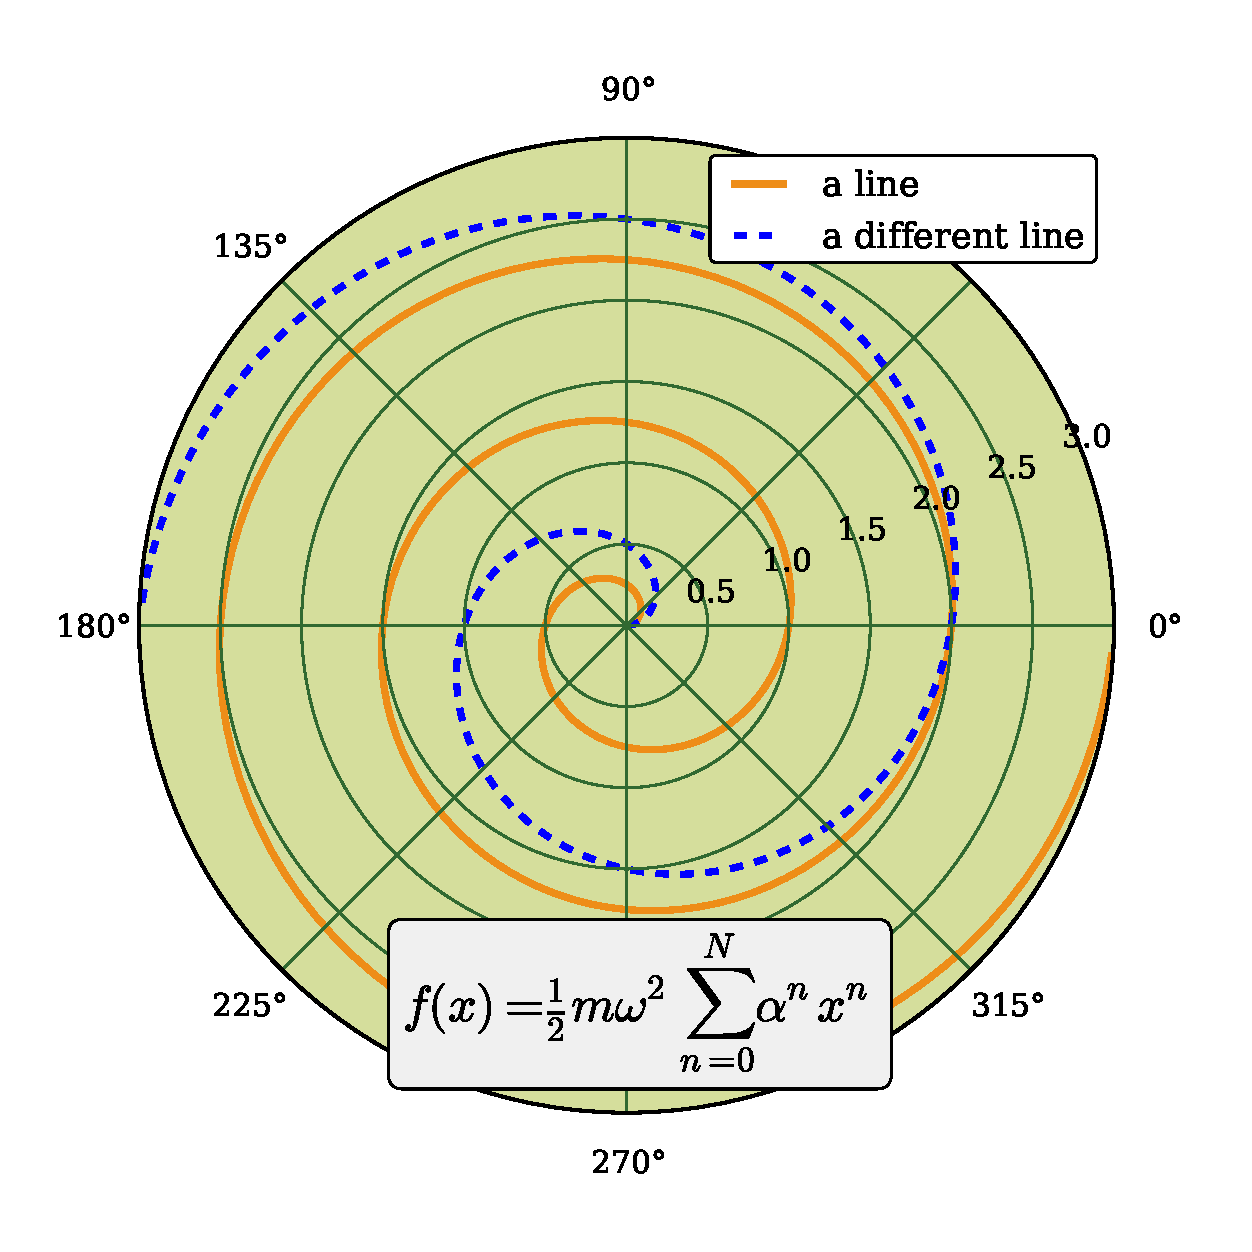
\includegraphics[width=\imsize]{cap2_f1}
\caption[La figura muestra algunas curvas m\'{a}s o menos lindas]{La figura muestra algunas curvas m\'{a}s o menos lindas. El gr\'{a}fico est\'{a} en coordenadas porlares como se muestra en la }
\end{figure}


\item Interpretaci\'{o}n de Copenhague, es la interpretaci\'{o}n probablemente m\'{a}s com\'{u}n y a la
  que se han adherido la mayor\'{\i}a de manuales de mec\'{a}nica cu\'{a}ntica tradicionalmente. Debida
  inicialmente a Niels Bohr y el grupo de f\'{\i}sicos que trabajaba con \'{e}l en Copenhague hacia
  1927. Se asume el principio de incertidumbre y el principio de complementariedad de las
  descripciones ondulatoria y corpuscular.
\item Interpretaci\'{o}n participatoria del principio antr\'{o}pico.
\item Interpretaci\'{o}n de historias consistentes.
\item Teor\'{\i}as de colapso objetivo.De acuerdo con estas teor\'{\i}as, la superposiciones de
  estados se destruyen aunque no se produzca observaci\'{o}n, difiriendo las teor\'{\i}as en qu\'{e}
  magnitud f\'{\i}sica es la que provoca la destrucci\'{o}n (tiempo, gravitaci\'{o}n,temperatura,
  t\'{e}rminos no lineales en el operador de evoluci\'{o}n...). Esa destrucci\'{o}n es lo que evita
  las ramas que aparecen en la teor\'{\i}a de los multi-universos o universos paralelos . La
  palabra "objetivo" procede de que en esta interpretaci\'{o}n tanto la funci\'{o}n de onda como
  el colapso de la misma son "reales", en el sentido ontol\'{o}gico.En la interpretaci\'{o}n de
  los muchos-mundos, el collapso no es objetivo, y en la de Copenhague es una hip\'{o}tesis
  ad-hoc.

  \begin{itemize}
  \item Interpretaci\'{o}n multiverso.
  \item Decoherencia por el entorno
  \item Interpretaci\'{o}n de Bohm
  \item Interpretaci\'{o}n Madhyamika
  \end{itemize}
\end{enumerate}

En la primera ecuaci\'{o}n
\begin{equation}
\phi_{1}(z)=A_{1}e^{ik_{1}z}+B_{1}e^{-ik_{1}z}.
\end{equation}

En la segunda ecuaci\'{o}n:
\begin{equation}
\phi_{2}(z)=A_{2}e^{ik_{2}z}+B_{2}e^{-ik_{2}z}.
\end{equation}

La soluci\'{o}n de la tercera ecuaci\'{o}n se puede obtener a partir de la
soluci\'{o}n en la primera ecuaci\'{o}n aplicando 
\begin{equation}
\phi_{3}(z)=e^{iKd}(A_{1}e^{ik_{1}(z-l)}+B_{1}e^{-ik_{1}(z-l)}).
\end{equation}

\chapter{otr}
\label{C:otr}

\section{Secci\'{o}n 1}
\label{S:seccion-1}

\section{otra}
\label{S:otra}

\section{una}
\label{S:una}

\section{dos}
\label{S:dos}

\section{tres}
\label{S:tres}

\chapter{cuatro}
\label{C:cuatro}

\section{una}
\label{S:una-1}

\section{otra mas}
\label{S:otra-mas}


%%% Local Variables: 
%%% mode: latex
%%% TeX-master: "template"
%%% End: 



\appendix
\chapter{Diferenciación numérica de datos ruidosos y no suaves}\label{C:ap1}
\chapterquote{Distinguishing the signal from the noise requires both scientific knowledge and self-knowledge: the serenity to accept the things we cannot predict, the courage to predict the things we can, and the wisdom to know the difference.}{Nate silver, 2012}
\graphicspath{{figs/apendice_derivada_ruidosa}}
%%%%%%%%%%%%%%%%%%%%%%%%%%%%%%%%%%%%%%%%%%%%%%%%%%%%%%%%%%%%%%%%%%%%%%%%




El cálculo de derivadas de datos de mediciones ruidosas es omnipresente en las ciencias físicas, de ingeniería y biológicas, y suele ser un paso fundamental en el desarrollo de modelos dinámicos o el diseño del control. Por desgracia, la formulación matemática de la diferenciación numérica suele estar mal planteada, y los investigadores recurren a menudo a un proceso ad hoc para elegir uno de los muchos métodos computacionales y sus parámetros \cite{9241009}. Existe un amplio y variado conjunto de herramientas matemáticas para estimar las derivadas de datos ruidosos, la mayoría de las cuales se formulan como un problema mal planteado regularizado por algunas restricciones de suavizado apropiadas.  En este apéndice se considera el problema de diferenciar una función especificada por datos ruidosos. El método  elegido es la \gls{regularizacion} del proceso de diferenciación el cual evita la amplificación de ruido de los métodos de diferencias finitas.  La regularización de variación total se utiliza por que permite soluciones discontinuas. El algoritmo simple resultante diferencia con precisión las funciones ruidosas, incluidas aquellas que tienen una derivada discontinua.

\section{Introducción}

En muchas aplicaciones científicas, es necesario calcular la derivada de funciones especificadas por datos. Las aproximaciones por diferencias finitas convencionales amplificarán en gran medida cualquier ruido presente en los datos. La eliminación del ruido de los datos antes o después de la diferenciación no suele dar resultados satisfactorios \cite{chartrand_numerical_2011}.  

Un método que da buenos resultados es regularizar el propio proceso de diferenciación. Esto garantiza que la derivada calculada tendrá cierto grado de regularidad, hasta un punto que a menudo se puede controlar ajustando los parámetros. Un marco común para ello es la regularización de Tikhonov \cite{1570291226450870144} del problema inverso correspondiente. Es decir, la derivada de una función  $f$ en  $[0,L]$ es el minimizador del funcional

\begin{equation}\label{eq:81}
F(u)=\alpha R(u) +DF\left(Au-f\right)
\end{equation}


donde  $R(u)$  es un término de regularización o penalización que penaliza la irregularidad en  $u$ , $Au(x)=\int_{0}^{x}u$  es el operador de antidiferenciación,  $DF\left(Au-f\right)$  es un término de fidelidad de los datos que penaliza la discrepancia entre $Au$ y $f$, y $\alpha$  es un parámetro de regularización que controla el equilibrio entre los dos términos.  El término de fidelidad de los datos $DF$ suele ser el cuadrado de la norma $L^2$, $DF=\int_{0}^{L} \left| \cdot \right|^2$ , como corresponde si $f$  tiene ruido gaussiano blanco aditivo. Se pueden utilizar otros términos de fidelidad de datos si el ruido tiene una distribución diferente y conocida.

\section{ Regularización de variación total }

La regularización de variación total se debe a Rudin et al. en \cite{rudin_nonlinear_1992}. Desde entonces ha encontrado muchas aplicaciones en el tratamiento de imágenes.  Chartrand \cite{chartrand_numerical_2011}  propuso  utilizar la regularización de variación total en la \cref{eq:81}. Así, se puede calcular  la derivada de  $f$  en  $[0,L]$  como el minimizador del funcional 

\begin{equation}\label{eq:82}
	F(u)=\alpha\int_{0}^{L}\left|u^\prime \right| +\frac{1}{2}\int_{0}^{L}\left| Au-f\right|^2. 
\end{equation}

Suponemos que $f\in L^2$ (una suposición vacía en el caso discreto), y por conveniencia que $f(0)=0$ (en la práctica simplemente restamos $f(0)$ de $f$ ). La función $F$ está definida en $BV[0,L]$, el espacio de funciones de variación acotada.   El uso de la variación total consigue dos cosas. Suprime el ruido, ya que una función ruidosa tendrá una variación total grande. Tampoco suprime las discontinuidades de salto, a diferencia de las regularizaciones típicas. Esto permite el cálculo de derivadas discontinuas y la detección de esquinas y bordes en datos ruidosos.

\section{Implementación numérica}

Un enfoque sencillo para minimizar \cref{eq:82} es el descenso del gradiente. Esto equivale a evolucionar a estacionariedad la EDP obtenida a partir de la ecuación de Euler-Lagrange:

\begin{equation}\label{eq:83}
u_t=\alpha\frac{d}{dx}\frac{u^\prime}{\left| u^\prime\right| }-A^T\left(Au-f\right),
\end{equation}

donde $A^Tv(x)=\int_{x}^{L}v$ es el $L^2$-adjunto de $A$. Sustituyendo $\left|u^\prime \right|$  en el denominador por $\sqrt{\left(u^\prime\right)^2+\epsilon}$ para algún valor pequeño de $\epsilon>0$  evita la división por cero. Típicamente, La \cref{eq:83} se implementa con marcha temporal explícita, con $u_t$  discretizada como $\left(u_{n+1}-u_n\right)/\Delta t$ para algún valor fijo de $\Delta t$. El problema con la \cref{eq:83}  es que la convergencia es lenta. Un algoritmo más rápido es el método de difusividad retardada de Vogel y Oman \cite{vogel_iterative_1996}. La idea es sustituir en cada iteración de  la \cref{eq:83}  el operador diferencial no lineal $u\mapsto(d/dx)\left(u^\prime/ \left|u^\prime \right|\right)$ por el operador lineal $u\mapsto(d/dx)\left(u^\prime/\left|u^\prime_n \right| \right)$ . Se ha demostrado que el algoritmo converge al minimizador de $F$.


Menos sencilla es la elección del parámetro de regularización $\alpha$. Un enfoque consiste en utilizar el principio de discrepancia: la diferencia cuadrática media entre $Au^*$ y $f$  debe ser igual a la varianza del ruido en  $f$ . Esto tiene el efecto de elegir la solución más regular del problema inverso mal planteado $Au=f$  que sea consistente con los datos  $f$ . En la práctica, el ruido en $f$  no suele conocerse, pero la varianza del ruido puede estimarse comparando $f$ con una versión suavizada de  $f$. El otro enfoque consiste simplemente en utilizar el método de ensayo y error, ajustando  $\alpha$  para obtener el equilibrio deseado entre la supresión de las oscilaciones y la fidelidad a los datos. En la siguiente sección, veremos un ejemplo que muestra el efecto del valor de $\alpha$.


\section{Ejemplo}

Para el calculo de la derivada numérica regularizada por variación total (TVDiff) se utilizo la implementación en Python realizada por Simone Sturniolo \footnote{La documentación esta disponible en \url{https://github.com/stur86/tvregdiff}}. Para ver el funcionamiento del algoritmo utilizamos  un ejemplo sencillo.  Sea $f_0(x)=\left| x-1/2\right|$ , definida en 100 puntos uniformemente espaciados en  $[0,1]$ . Obtenemos  $f$  añadiendo ruido gaussiano de desviación estándar $0.05$. La \cref{f:funcion_ruidosa} muestra el  $f$ . En primer lugar, mostramos en la \cref{f:derivada_centrada} el resultado de calcular  $u(x)=df/dx$ por diferencias finitas. Comparamos los resultados con la derivada verdadera  $u(x)=sgn(x)$ y una aplicación ingenua de diferencias finitas $u_{FDM}$. Incluso  con un ruido de amplitud moderada como el de este ejemplo, una aplicación ingenua como lo es $u_{FDM}$ produce estimaciones de la derivada que son demasiado ruidosas para ser útiles.


\begin{figure}[h!]
\centering{}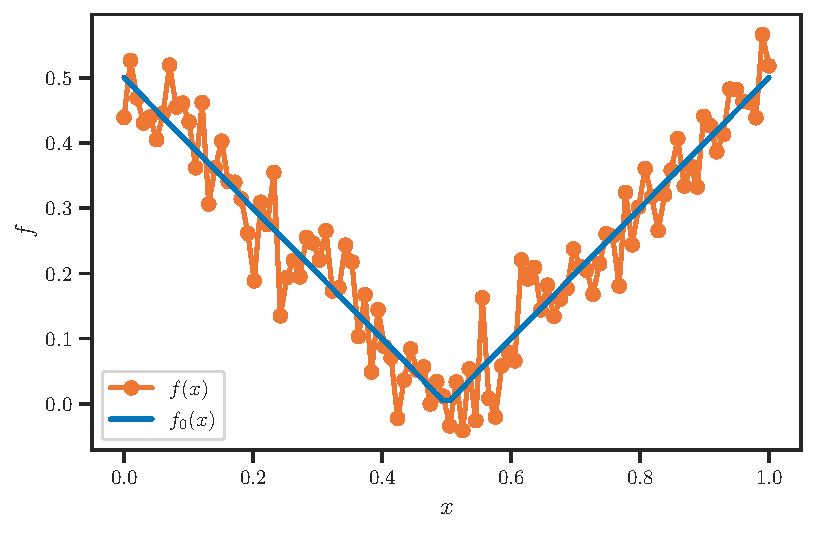
\includegraphics[width=\imsize]{funcion_ruidosa.pdf}
\caption{La función $f$ obtenida a partir de  $f_0=\left| x-1/2\right|$   añadiendo ruido gaussiano de desviación estándar $0.05$}\label{f:funcion_ruidosa}  
\end{figure}

\begin{figure}[h!]
	\centering{}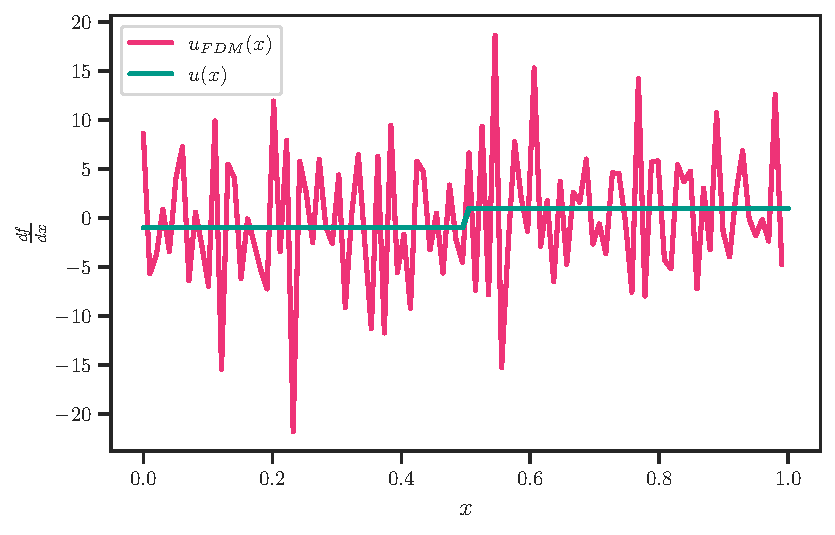
\includegraphics[width=\imsize]{derivada_centrada.pdf}
	\caption{El cálculo de $u_{FDM}(x)$ con diferencias finitas amplifica enormemente el ruido.}\label{f:derivada_centrada}  
\end{figure}


Ahora, se implementa la TVDiff, dada por la \cref{eq:82}. Para ver como varían los resultados con el parámetro de regularización $\alpha$, se comparan 3 valores de este. En todos los casos se utilizan los parámetros $\epsilon=$\num{1e-6} y 7000 iteraciones.  Con un   $\alpha=$\num{1e-4}  tan bajo (Figura (a)) el ruido residual en el proceso de diferenciación aún se amplifica lo suficiente como para dar un resultado insatisfactorio. Con una regularización más fuerte $\alpha=2$ el resultado es mucho mas suave y similar al resultado teórico.  A pesar de la fuerte suavización, se captan bien las rápidas subidas y bajadas del derivado. Éste es el efecto de la regularización, cuya elección sirve para determinar la magnitud de la fluctuación que se considera insignificante. Aunque el suavizado mitiga los errores, también puede introducir sesgos.  Finalmente un parámetro mas optimizo seria $\alpha=0.2$, la forma general de $f^\prime_0$ se captura casi perfectamente. El salto está correctamente localizado. La única imprecisión es el tamaño del salto: hay una pérdida de contraste, típica de la regularización de totalización en presencia de ruido. Disminuir el tamaño del salto reduce el término de penalización en la \cref{eq:82}, a expensas de aumentar el término de fidelidad de los datos.


\begin{figure}[h!]
	\centering{}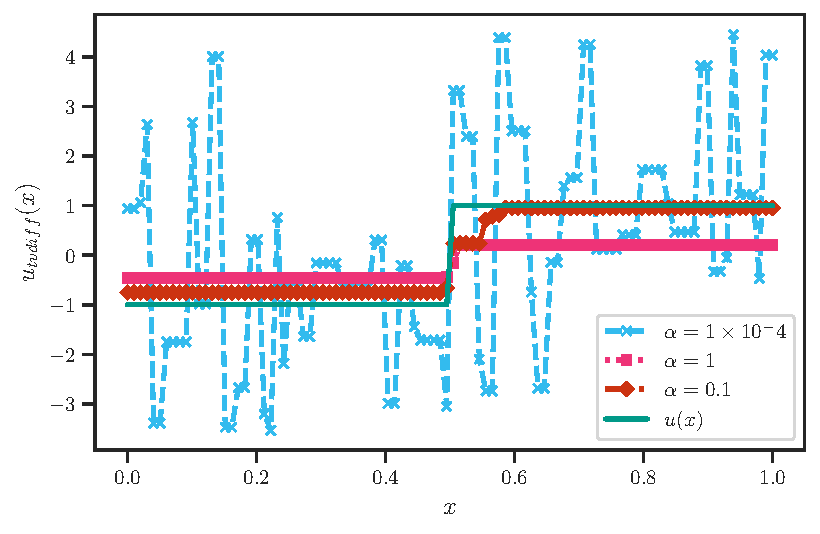
\includegraphics[width=\imsize]{derivada_regularizadas.pdf}
	\caption[Resultados de la derivada con diversos valores del parámetro de regularización. ]{Resultados de la derivada con diversos valores del parámetro de regularización. Los resultados se comparan con el valor teórico $u(x)$ que en este grafico es la linea color verde. Con un parámetro de regularización bajo $\alpha=0.1$ (linea color celeste) el resultado es ruidoso e impreciso.  Por otra parte un parámetro alto $\alpha=1$ de regularización puede introducir sesgos (linea color rosa). Una regularización optima  con $\alpha=0.1$  produce una derivada sin ruido con un salto agudo correctamente localizado. La discrepancia de los valores de  $\pm 1$  se deben a la pérdida de contraste, un artefacto de los métodos de variación total en presencia de ruido.}\label{f:derivada_regularizada}  
\end{figure}


También se muestra el resultado de aplicar el operador de antidiferenciación al valor de las derivadas calculadas (\cref{f:integral_derivada_regularizada}) y lo comparamos con el de la teórica. Como sucede en la derivada el mejor resultado es cuando $\alpha=0.1$. 


\begin{figure}[h!]
	\centering{}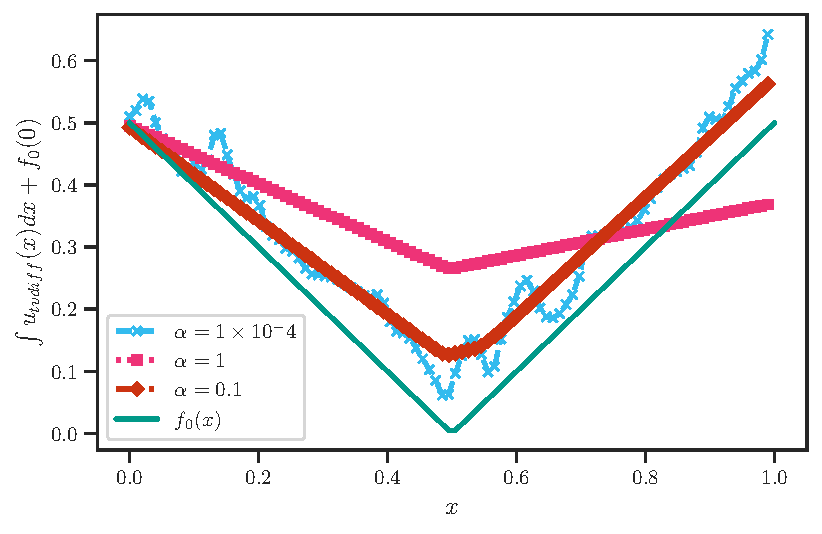
\includegraphics[width=\imsize]{integral_derivada_regularizadas.pdf}
	\caption[Resultados de la anti-derivada aplicada la derivada regularizada con diversos valores del parámetro de regularización. ]{Resultados de la anti-derivada aplicada la derivada regularizada  con diversos valores del parámetro de regularización. Los resultados se comparan con el valor real $f_0(x)$ que en este grafico es la linea color verde. Con un parámetro de regularización bajo $\alpha=0.1$ (linea color celeste) se obtiene una función ruidosa tal como $f(x)$.  Por otra parte un parámetro alto $\alpha=1$ de regularización puede introducir sesgos (linea color rosa) el cual desviá el resultado de la función real. Una regularización mas optima  como $\alpha=0.1$  produce un resultado  muy similar a la función exacta $f_0$}\label{f:integral_derivada_regularizada}  
\end{figure}

\section{Elección de parámetros óptimos}\label{sec:parametors_optimos}

Como se explico en la anterior sección para obtener un resultado optimo se debe realizar una elección adecuada de los parámetros. Se debe buscar que el valor de este parámetro no sea muy alto  lo cual suavizaría la derivada  en exceso dando como resultado  perdidas de información que pueden ser relevantes.  Por otra parte  un parámetro demasiado bajo al igual que las diferencias finitas da un resultado  ruidoso. Sin embargo, el nivel y el tipo de regularización suelen imponerse de forma ad hoc, por lo que actualmente no existe un \textquote{mejor método} consensuado para obtener las derivadas \textquote{mejor ajustadas}. Para solventar este problema  Van Breugel et al \cite{van_breugel_numerical_2020} adoptaron un enfoque basado en principios y propusieron  un marco de optimización multiobjetivo para elegir los parámetros que minimizan una función de pérdida para equilibrar la fidelidad y la suavidad de la estimación de la derivada. Este  marco presenta tres ventajas significativas. En primer lugar, la tarea de seleccionar múltiples parámetros se reduce a la elección de un único hiperparámetro. En segundo lugar, cuando se desconocen los datos reales, se proporciona una heurística para seleccionar este hiperparámetro basándonos en el espectro de potencia y la resolución temporal de los datos. En tercer lugar, el valor óptimo del hiperparámetro es coherente con los distintos métodos de diferenciación, por lo que este enfoque unifica métodos de diferenciación numérica muy diferentes y facilita la comparación imparcial de sus resultados. Por último, se proporciona una amplia biblioteca Python de código abierto, pynumdiff \footnote{La documentación se puede encontrar en  el siguiente link \url{https://github.com/florisvb/PyNumDiff}}, para facilitar su aplicación a diversos conjuntos de datos. El  objetivo de este paquete es desarrollar un enfoque general para elegir metódicamente parámetros que equilibren la necesidad de minimizar tanto el error como el sesgo. 

Para lograr este objetivo se minimiza una función de pérdida consistente en una suma ponderada de dos métricas calculadas a partir de la estimación de la derivada $\hat{\dot{x}}$: la fidelidad de la integral de la derivada y su suavidad. El procedimiento es el siguiente:  dadas unas mediciones ruidosas $y$, buscamos estimar la derivada en el tiempo del sistema dinámico que subyace a las mediciones $\hat{\dot{x}}$ . Cuando la verdadera $\dot{x}$ es desconocida, proponemos elegir el conjunto de parámetros $\Phi$ (para cualquier algoritmo numérico dado)   que minimicen la siguiente función de pérdida, 

\begin{equation}\label{eq:ap:1}
	L = \text {RMSE} \bigg (\text {trapz}({\hat {\dot {\mathbf {x}}}} (\Phi)) + \mu, {\mathbf {y}} \bigg) + \gamma \bigg ({TV}\big ({\hat {\dot {\mathbf {x}}}} (\Phi)\big)\bigg),\qquad 
\end{equation}


donde  RMSE es el error cuadrático medio,

\begin{equation}
\text {RMSE}({\hat {\dot {\mathbf {x}}}}, {\dot {\mathbf {x}}}) = \lVert ({\hat {\dot {\mathbf {x}}}} - {\dot {\mathbf {x}}})\rVert _{2},
\end{equation}

$\lVert{\cdot}\rVert _{2}$ es la 2-norma  del vector.  $\text{trapz}(\cdot)$ es la integral numérica trapezoidal en tiempo discreto, $\mu$ resuelve la constante de integración desconocida, 

\begin{equation} 
	\mu =\frac {1}{m}\sum _{k=0}^{m}\bigg (\text {trapz}({\hat {\dot {\mathbf {x}}}} (\Phi)) - {\mathbf {y}} \bigg),
	\end{equation}
	
$\gamma$ es un hiperparámetro y   $TV$ es la variación total,

\begin{equation} \label{eq:ap:2}
	TV({\hat {\dot {\mathbf {x}}}}) = \frac {1}{m}\left \lVert{ {\hat {\dot {\mathbf {x}}}} _{0:m-1}- {\hat {\dot {\mathbf {x}}}} _{1:m}}\right \rVert _{1},
	\end{equation}
	
 $\left\lVert{\cdot}\right\rVert _{1}$  denota la norma $\ell_1$ y $m$ es el número de instantáneas temporales de los datos.  El primer término de la función de pérdida en la\Cref{eq:ap:1} promueve la fidelidad de la estimación de la derivada asegurando que la integral de la estimación de la derivada se mantiene similar a los datos, mientras que el segundo término promueve la suavidad de la estimación de la derivada. Si $\gamma$ es cero, la función de pérdida simplemente devuelve la derivada por diferencias finitas. Los valores altos de $\gamma$ darán como resultado una estimación de la derivada más suave.  Esta función de pérdida reduce efectivamente el conjunto de parámetros $\Phi$ (que oscila entre 1 y 3 o más, dependiendo del método) a un único hiperparámetro $\gamma$. Desafortunadamente, $L$ no es convexo, pero se pueden utilizar rutinas de optimización manejables para resolver el conjunto de $\phi$ que minimizan $L$. Aquí se utiliza el método de Nelder-Mead \cite{nelder_simplex_1965}, un método de búsqueda directa simplex descendente que funciona bien para problemas de optimización no lineal. Para evitar que la optimización converja en mínimos incorrectos, lo utilizamos con múltiples condiciones iniciales. Finalmente este enfoque sugiere estas métricas como aproximaciones para minimizar el error y el sesgo de la derivada estimada, y en el articulo \cite{van_breugel_numerical_2020}  se demuestra que el barrido a través de los valores de un único hiperparámetro $\gamma$ produce estimaciones de la derivada que generalmente trazan el frente de Pareto de soluciones que minimizan el error y el sesgo.  Es importante destacar que este marco de optimización no asume ningún conocimiento de la verdadera derivada subyacente y reduce la tarea de seleccionar muchos parámetros de cualquier algoritmo de diferenciación a la resolución de una función de pérdida con un único hiperparámetro. 





%%% Local Variables: 
%%% mode: latex
%%% TeX-master: "template"
%%% End: 


\begin{biblio}
\bibliography{mibib}
\end{biblio}


\begin{postliminary}

\begin{seccion}{Publicaciones asociadas}
  \begin{enumerate}
  \item Mi primer aviso en la revista \textbf{ABC}, 1996
  \item Mi segunda publicaci\'{o}n en la revista \textbf{ABC}, 1997
  \end{enumerate}
\end{seccion}

\begin{seccion}{Agradecimientos}
A todos los que se lo merecen, por merecerlo
\end{seccion}

\end{postliminary}

\end{document}

